%% %%=================================================================
%% %% <UTF-8>
%% %% 北航学位论文模板使用样例
%% %% 请将以下文件与此LaTeX文件放在同一目录中.
%% %%-----------
%% %% buaa.cls                  : LaTeX宏模板文件
%% %% bst/GBT7714-2005.bst      : 国标参考文献BibTeX样式文件2005(https://github.com/Haixing-Hu/GBT7714-2005-BibTeX-Style)
%% %% bst/GBT7714-2015.bst      : 国标参考文献BibTeX样式文件2015(https://github.com/zepinglee/gbt7714-bibtex-style)
%% %% pic/logo-buaa.eps         : 论文封皮北航字样
%% %% pic/head-doctor.eps       : 论文封皮学术博士学位论文标题(华文行楷字体替代解决方案)
%% %% pic/head-prodoctor.eps    : 论文封皮专业博士学位论文标题(华文行楷字体替代解决方案)
%% %% pic/head-master.eps       : 论文封皮学术硕士学位论文标题(华文行楷字体替代解决方案)
%% %% pic/head-professional.eps : 论文封皮专业硕士学位论文标题(华文行楷字体替代解决方案)
%% %% tex/*.tex                 : 本模板样例中的独立章节
%% %%-----------
%% %% 请统一使用UTF-8编码.
%% %%=================================================================

%=================================================================
% buaa基于ctexbook模板
% 论文样式参考自《研究生手册--二〇二〇年七月》
%======================
% 模板导入:
% \documentclass[thesis,permission,printtype,ostype,<ctexbookoptions>]{buaa}
%======================
% 模板选项:
%======================
% I.论文类型(thesis)
%--------------------
% a.学术硕士论文(master)[缺省值]
% b.专业硕士论文(professional)
% c.学术博士论文(doctor)
% d.专业博士论文(prodoctor)
%--------------------
% II.密级(permission)
%--------------------
% a.公开(public)[缺省值]
% b.内部(privacy)
% c.秘密(secret=secret3)
% c.1.秘密3年(secret3)
% c.2.秘密5年(secret5)
% c.3.秘密10年(secret10)
% c.4.秘密永久(secret*)
% d.机密(classified=classified5)
% d.1.机密3年(classified3)
% d.2.机密5年(classified5)
% d.3.机密10年(classified10)
% d.4.机密永久(classified*)
% e.绝密(topsecret=topsecret10)
% e.1.绝密3年(topsecret3)
% e.2.绝密5年(topsecret5)
% e.3.绝密10年(topsecret10)
% e.4.绝密永久(topsecret*)
%--------------------
% III.打印设置(printtype)
%--------------------
% a.单面打印(oneside)[缺省值]
% b.双面打印(twoside)
%--------------------
% IV.系统类型(ostype)
%--------------------
% a.win(oneside)[缺省值]
% b.linux (linux)
% c.mac (mac)
%--------------------
% V.ctexbook设置选项(<ctexbookoptions>)
%--------------------
% ...
%======================
% 其他说明:
% 1. Mac系统请使用mac选项,并使用XeLaTeX编译。
% 2. 可加入额外ctexbook文档类的选项,其将会被传递给ctexbook。
%    例如:\documentclass[fontset=founder]{buaa}
% 3. CTeX在Linux下默认使用Fandol字体,为避免某些生僻字无法显示,在系统已安装方正
%    字体的前提下可通过fontset=founder选项常用方正字体。
%=================================================================

% !TeX program = xelatex

\documentclass[master,privacy,oneside,win]{buaa}

%=================================================================
% 开启/关闭引用编号颜色:参考文献,公式,图,表,算法 等……
\refcolor{off}   % 开启: on[默认]; 关闭: off;
% 摘要和正文从右侧页开始
\beginright{off} % 开启: on[默认]; 关闭: off;
% 空白页留字
% \emptypagewords{[ -- This page is a preset empty page -- ]}

%=================================================================
% buaa模板已内嵌以下LaTeX工具包:
%--------------------
% ifthen, etoolbox, titletoc, remreset,
% geometry, fancyhdr, setspace,
% float, graphicx, subfigure, epstopdf,
% array, enumitem,
% booktabs, longtable, multirow, caption,
% listings, algorithm2e, amsmath, amsthm,
% hyperref, pifont, color, soul,
% ---
% For Win: times
% For Lin: newtxtext, newtxmath
% For Mac: times, fontspec
%--------------------
% 请在此处添加额外工具包>>


%=================================================================
% buaa模板已内嵌以下LaTeX宏:
%--------------------
% \highlight{text} % 黄色高亮
%--------------------
% 请在此处添加自定义宏>>


%%=================================================================
% 论文题目及副标题-{中文}{英文}
\Title{基于Transformer的知识图谱补全算法研究}{Research of Knowledge Graph Completion Algorithm Based on Transformer}
% \Subtitle{版本 \BUAAThesisVer{}}{Version \BUAAThesisVer{}}

% 学科大类,默认工学
% \Branch{工学}

% 院系,专业及研究方向
\Department{软件学院}
\Major{软件工程}
\Feild{软件工程}

% 导师信息-{中文名}{英文名}{职称}
\Tutor{谭火彬}{Tan Huobin}{副教授}
% \Cotutor{副导师姓名}{Cotutor}{高工}

% 学生姓名-{中文名}{英文名}
\Author{朱桐}{Zhu Tong}
% 学生学号
\StudentID{SY2121127}

% 中图分类号
\CLC{TP391.4}

% 时间节点-{月}{日}{年}
\DateEnroll{09}{01}{2021}
\DateGraduate{05}{16}{2024}
\DateSubmit{01}{10}{2024}
\DateDefence{03}{01}{2024}

%%=================================================================
% 摘要-{中文}{英文}
\Abstract{%
  摘要是学位论文内容的简短陈述,应体现论文工作的核心思想。论文摘要应力求语言精炼准确。博士学位论文的中文摘要一般约800$\sim$1200字;硕士学位论文的中文摘要一般约500字。摘要内容应涉及本项科研工作的目的和意义、研究思想和方法、研究成果和结论。博士学位论文必须突出论文的创造性成果,硕士学位论文必须突出论文的新见解。

  关键字是为用户查找文献,从文中选取出来揭示全文主体内容的一组词语或术语,应尽量采用词表中的规范词(参考相应的技术术语标准)。关键词一般3$\sim$5个,按词条的外延层次排列(外延大的排在前面)。关键词之间用逗号分开,最后一个关键词后不打标点符号。

  为了国际交流的需要,论文必须有英文摘要。英文摘要的内容及关键词应与中文摘要及关键词一致,要符合英语语法,语句通顺,文字流畅。英文和汉语拼音一律为Times New Roman体,字号与中文摘要相同。
  }{%
  What were you doing 500 years ago? Oh, that's right nothing, because you didn't exist yet. In fact, several generations of your family had yet to leave their mark on the world, but one very special shark may already have been swimming in the chilly North Atlantic at that time, and the incredible animal is somehow still alive today.

  Scientists studying Greenland sharks observed the particularly old specimen just recently, and after studying it they've determined that the creature is approximately 272 to 512 years old. That's an absolutely insane figure, and if its age lands towards the higher end, it makes the animal the oldest observed living vertebrate on the entire planet.

  Greenland sharks are an incredible species in a number of ways, but most notable is its longevity. The sharks are well over 100 years old before even reaching sexual maturity, and regularly live for centuries. This particularly old specimen, along with 27 others, were analyzed using radiocarbon dating. The reading came back at around 392 years, but potential margin of error means the animal's true age is somewhere between 272 and 512.

  The shark, which is a female, measures an impressive 18 feet long. That's pretty large, but it might not sound particularly large for an ocean-dwelling creature that lives hundreds of years. That is, until you consider that the Greenland shark only grows around one centimeter per year. With that in mind, 18 feet is actually downright massive.

  As for how this particular shark species manages to live so incredibly long, scientists attribute a lot of its longevity to its sluggish metabolism, as well as its environment. The frigid waters where the sharks thrive is thought to increase overall lifespan in a variety of ways. Past research has shown that cold environments can help slow aging, and these centuries-old sharks are most certainly benefiting from their chilly surroundings.

  --- Online news {\it Scientists find incredible shark that may be over 500 years old and still kicking\/}, 12.16.2017. (http://bgr.com/2017/12/14/oldest-shark-greenland-512-years-old/).
}
% 关键字-{中文}{英文}
\Keyword{%
    北航,学位论文,博士,硕士,中文,\LaTeX{}模板,\BUAAThesis{}
  }{%
    News, BGR, Shark
}

% 图标目录
\Listfigtab{on} % 启用: on[默认]; 双标题:bi; 关闭: off;

% 缩写定义 按tabular环境或其他列表环境编写
% \Abbreviations{ \centering
% \begin{tabular}{cl}
%   $E$ & 能量 \\
%   $m$ & 质量 \\
%   $c$ & 光速 \\
%   $P$ & 概率 \\
%   $T$ & 时间 \\
%   $v$ & 速度 \\
% \end{tabular}
% }

\begin{document}

%%=================================================================
% 标题级别
%--------------------
% \chapter{第一章}
% \section{1.1 小节}
% \subsection{1.1.1 条}
% \subsubsection{1.1.1.1}
% \paragraph{1.1.1.1.1}
% \subparagraph{1.1.1.1.1.1}
%--------------------
%%=================================================================

% 绪论
\chapter{绪论}

\section{研究背景与意义}
论文选题来源于实验室承担的国家重点研发计划等多个课题,需要面向材料、建筑等不同领域场景建立行业知识图谱。本文主要研究高效的知识图谱补全算法,为课题中各类行业知识图谱的构建和下游任务的应用提供理论和技术支撑。

知识图谱(Knowledge Graph, KG)是知识库的一种主要形式,是由事实三元组(头实体、关系、尾实体)表示的结构化知识的集合,在多个人工智能领域中得到了广泛的应用,例如语义搜索\upcite{yuyisousuo}、问答\upcite{wenda}和推荐系统\upcite{recommendation_system}。主流的开放知识图谱包括FreeBase\upcite{freebase},Wikidata\upcite{Wikidata},DBpedia\upcite{DBpedia}和YAGO\upcite{YAGO}等,它们通常包含由数十亿个实体和关系所构建的海量事实。然而,由于现实世界不断发展带来的知识的动态变化,即使是大规模知识图谱也难以囊括所有的知识,这限制了知识图谱在现实世界中的应用。因此,近年知识图谱补全(Knowledge Graph Completion, KGC),又称链路预测任务,成为了知识图谱领域的热门研究方向,尝试在给定事实三元组中的头(尾)实体和关系的情况下,自动预测缺失的尾(头)实体。

% 论文选题来源于国家重点研发计划课题“稀土催化材料专用数据库及全流程数字化研发平台”,本文研究高效的知识图谱补全方法,为稀土催化材料知识图谱构建和应用提供技术支撑。

% 稀土是由镧系元素和与其密切相关的钪和钇等化学元素组成,稀土的存在能有效提高催化剂的储氧能力、提高活性金属的分散度、降低贵金属用量、促进水气转化和蒸汽重整反应等性质,在催化材料领域中有着重要的应用。
% % 知识图谱(Knowledge Graph, KG)是知识库的一种主要表现形式,是由事实三元组(头实体、关系、尾实体)表示的结构化知识的集合,在多个领域中已经得到了广泛的应用。
% 稀土催化材料知识图谱存储着稀土催化材料的合成方式、理化性质、组成结构等重要信息,被应用于稀土催化材料合成等任务中,能够帮助稀土催化材料降低开发成本、减少开发周期。然而,由于稀土材料领域的不断研究发展带来的知识的动态变化,和大多数知识图谱一样,稀土催化材料知识图谱往往是不完全的,难以囊括领域内的所有知识,对其在上层任务中的应用造成了阻碍。因此,为了挖掘图谱内蕴含的丰富信息,完善稀土催化材料知识图谱,知识图谱补全(Knowledge Graph Completion, KGC),又称链路预测任务,成为了知识图谱领域的热门研究方向。

知识图谱补全需要挖掘图谱中隐藏的语义信息,但是知识图谱中的事实三元组一般是以文本形式进行储存的,无法直接利用,需要首先寻找一种合适的方式来对语义信息进行表达。传统方法一般通过特征工程进行,效率低且可移植性较差,因此不少研究者投入了自动化知识补全的研究。

目前,知识图谱补全的主流解决方案是知识图谱嵌入(Knowledge Graph Embedding, KGE),又称知识图谱表示学习\upcite{TransE}(Knowledge Graph Representation Learning)。它的核心思想是将图谱中的实体和关系投影到低维向量空间中,通过预先设计好的得分函数(Scoring Function)评估事实三元组的合理性,并基于知识图谱中的已有事实,最大化对正确事实三元组的预测概率。通过这种方式获得的嵌入表示不仅可以用于知识图谱补全,还能够用于语义搜索、问答和推荐系统等下游任务中。

传统的知识图谱表示学习方法主要考虑如何在单纯的三元组上进行学习,但这种方式存在较大的缺陷:
% 知识图谱本身是一个带标签的有向图,单纯考虑三元组的方法忽略了三元组之间的联系,
忽略了知识图谱本身的图结构信息。基于图神经网络的模型通过学习中心实体的局部邻域结构一定程度上解决了以上的问题,获得了更加优秀的性能,但依然存在不足:首先图神经网络的网络结构较浅,限制了模型的表达能力;另外,
% 基于图神经网络的方法的感受域与其网络层数相关,随着图神经网络层数的增加,相邻节点的感受域重叠程度升高,现有的方法会遭遇过度平滑的问题而导致性能下降,
基于图神经网络的方法随着网络层数的提升会遭遇过度平滑\upcite{over-smoothing}的问题,导致其只能捕捉单个实体附近1-2跳内的局部邻域信息,缺乏利用长距离依赖的能力。针对以上问题,本文研究基于Transformer的知识图谱补全方法。Transformer\upcite{Transformer}被公认为是建模序列数据的最强大的神经网络,不少工作致力于研究将Transformer网络应用到知识图谱嵌入工作中。本文研究利用Transformer强大的表达能力,结合知识图谱中图结构信息,实现更加准确的知识图谱补全,支持各类行业知识图谱的构建和应用。


\section{国内外研究现状}
知识图谱(Knowledge Graph, KG)的现代含义由2012年谷歌知识图谱\upcite{googlekg}的发布而确立,它是知识库的一种主要表现形式,是由事实三元组(头实体、关系、尾实体)表示的结构化知识的集合。图谱中的节点为实体,表示现实世界中的具体事物;图谱中的节点为关系,表示实体之间的联系。目前知识图谱已经在多个人工智能领域中得到了广泛的应用,例如语义搜索\upcite{yuyisousuo}、问答\upcite{wenda}和推荐系统\upcite{recommendation_system}。主流的开放知识图谱包括FreeBase\upcite{freebase},Wikidata\upcite{Wikidata},DBpedia\upcite{DBpedia}和YAGO\upcite{YAGO}等,它们通常包含使用数十亿个实体和关系构建的大量事实。然而由于现实世界不断发展,随时都有新的知识产生和旧的知识失效,即使是大规模知识图谱也不可避免的缺乏部分事实,这限制了知识图谱在现实世界中的应用。因此,近年知识图谱补全又称链路预测任务,成为了知识图谱领域的热门研究方向,尝试在给定事实三元组中的头(尾)实体和关系的情况下,自动预测缺失的尾(头)实体。

目前,知识图谱嵌入是知识图谱补全任务的主流解决方案,它将图谱中的实体和关系转化为低维向量空间中的向量,尽可能地保留其原始的结构性质,并用得分函数估计事实三元组正确的概率。现阶段对于知识图谱嵌入算法的研究,根据方法的核心思想和实现方式的不同,可以划分为传统的知识图谱嵌入方法,基于图神经网络的知识图谱嵌入方法,基于Transformer的知识图谱嵌入方法和融合多源信息的知识图谱嵌入方法。
\subsection{传统的知识图谱嵌入方法}
传统的知识图谱嵌入方法仅独立研究知识图谱中的事实三元组,主要包含基于翻译的方法、基于张量分解的方法和引入神经网络后的基于多层神经网络方法、基于卷积神经网络的方法。

基于翻译的方法是最早被提出的一类知识图谱嵌入方法,最早起源于2013年的TransE\upcite{TransE}模型,核心思想是将知识图谱中的关系视为一个实体到另一个实体的翻译,又被称为平移距离模型。由于TransE无法有效建模知识图谱中的一对多、多对一、多对多关系,后续基于TransE进行改进并衍生出了如TransH\upcite{TransH}、TransR\upcite{TransR}、TransD\upcite{TransD}等模型,不断丰富模型的表达能力。基于翻译的方法最大的优点在于其模型结构简单、计算速度快、易于理解且可解释性较强,但浅层的模型结构也限制了模型的表达能力。

以RESCAL\upcite{RESCAL}为代表的基于张量分解的方法则将整个知识图谱表示为一个高维的稀疏张量,通过对其进行张量分解来获得实体和关系的嵌入。RESCAL用一个维度为$N\times N\times M$的张量来表示一个实体数量为$N$,关系数量为$M$的知识图谱,通过对其进行张量分解,模型最终能够得到用一维向量表示的实体嵌入和用二维矩阵表示的关系嵌入。继RESCAL之后,基于张量分解的思想提出的DistMult\upcite{DistMult}、ComplEx\upcite{ComplEx}、ANALOGY\upcite{ANALOGY}等一系列模型分别从强化模型表达能力以及压缩模型参数两方面对RESCAL模型进行了改进。
% DistMult将关系嵌入进行了简化,选用了对角矩阵替代了RESCAL的二维矩阵,降低了模型的复杂度并获得了更优的性能;ComplEx则将模型从实数域扩展到了复数域,提高了模型的表达能力。
总的来说,基于张量分解的方法可解释性较强,并能够捕捉到实体和关系之间的双线性关系,但和基于翻译的方法类似,浅层的模型结构很难有效的学习图谱中蕴含的复杂信息,模型表达能力较弱。

而随着神经网络的发展,大量基于神经网络的知识图谱嵌入方法开始涌现。使用神经网络进行知识图谱嵌入能够建立更加复杂的模型,模型的表达能力更强,并且可以自动学习知识图谱当中蕴含的特征。这其中最早被提出的是基于多层神经网络的方法,SME\upcite{SME}、NTN\upcite{NTN}、MLP\upcite{MLP}等模型直接使用多层的神经网络去拟合知识图谱。
% 以事实三元组的嵌入作为模型的输入,输出三元组正确的概率。
这类方法相较之前没有神经网络结构的方法在性能上有了提升,但网络结构相对简单,可解释性较差。



而随后受到计算机视觉领域的研究方法的启发,有不少工作尝试引入卷积操作,大量基于卷积神经网络的方法被提出,其中最具代表性的方法为ConvE\upcite{ConvE}。ConvE将事实三元组中的头实体和关系的一维向量嵌入,重组为二维张量并对其进行卷积操作,将结果向量化之后经过神经网络层,随后和候选实体的嵌入进行点乘,输出事实三元组的正确概率。基于ConvE的思想,有不少方法提出了进一步的改进。ConvR\upcite{ConvR}使用关系嵌入构造卷积核,减少了网络的参数;ConvKB\upcite{ConvKB}通过在实体和关系的相同维度上进行卷积,能够捕获在实体和关系之间相同维度上的联系;InteractE\upcite{InteractE}则优化了二维张量的塑造方式,大大提升了头实体和关系之间的交互。

\subsection{基于图神经网络的知识图谱嵌入方法}

以上提到的知识图谱嵌入方法研究的对象是知识图谱中独立的三元组,这导致这些模型忽略了知识图谱的结构信息,因此被统一归类为传统的知识图谱嵌入方法。例如,这些方法没有办法感知到头实体的邻居实体,无法充分利用每个实体丰富的邻域结构,不仅链路预测的性能受到限制,而且也缺乏嵌入空间的可解释性。而基于图神经网络(Graph Neural Network, GNN)的知识图谱嵌入方法则利用图卷积神经网络来捕获图谱中的图结构信息,中心实体接受来自邻居实体与邻居关系的消息,并依此对实体和关系的嵌入表示进行更新。

R-GCN\upcite{R-GCN}是第一个利用图卷积神经网络学习知识图谱表示的方法,整体采用编码器-解码器架构。编码器部分通过图神经网络对图结构进行建模,在R-GCN的信息传播过程中,中心实体会接受来自出边、入边和自循环边三个方向的信息;通过多次信息传播模型能够获得多阶邻居的信息。解码器部分则基于编码的信息对三元组进行打分。后续提出的基于图神经网络的方法沿用了R-GCN的编码器-解码器架构,并在此基础上进行改进。SACN\upcite{SACN}模型基于关系类型将实体的邻域划分为带权值的子图进行聚合。TransGCN\upcite{TransGCN}提出了两种基于翻译的思想的编码器同时学习实体和关系嵌入,分别用于实数域和复数域。

而受到自然语言处理和计算机视觉领域中注意力机制的成功的启发,有不少工作尝试将注意力机制引入到基于图神经网络的知识图谱嵌入方法中来并取得了不错的效果。KBGAT\upcite{KBGAT}是首个在知识图谱嵌入领域应用图注意力网络的方法,模型能够自动分辨出哪些邻居实体的信息对于中心实体是更加重要的。RGHAT\upcite{RGHAT}将注意力机制进行了进一步的细分,引入了关系注意力机制和实体注意力机制,实现了更细粒度的建模。EIGAT\upcite{EIGAT}则通过随机游走算法引入了全局实体重要性,将局部注意力机制和知识图谱的全局信息进行了结合。

% 基于图神经网络的方法的成功证明了实体的局部邻域蕴含了丰富的信息,但知识图谱的结构信息除了常见的局部邻域之外还有多种表达形式,例如图路径和子图等。在知识图谱中,图路径被定义为图谱中的实体-关系链,例如(Yao Ming, Born In, Shanghai, City Of, China)。和基于图神经网络的方法利用中心实体的局部邻域进行链路预测不同,基于图路径的方法尝试利用知识图谱中的图路径信息来捕获实体与实体之间的长距离依赖。TransE-Comp和PTransE尝试建模两个实体之间的图路径上多跳关系构成的复合关系。Chain和RSN则对循环神经网络(Recurrent Neural Network, RNN)进行了改造,以学习图路径上的所有相邻实体和关系信息之间的依赖。Interstellar分析了挖掘图路径信息的重要性,并将知识图谱图路径学习问题定义为RNN神经网络架构搜索问题,并设计了一种特定于知识图谱嵌入领域的混合搜索算法以及搜索空间。

\subsection{基于Transformer的知识图谱嵌入方法}
基于图神经网络的方法通过对实体的邻域结构进行学习从而获得了阶段性的成功,性能普遍优于传统的知识图谱嵌入模型。但是图神经网络的表达能力虽然相较于传统方法的多层神经网络和卷积神经网络有了较大的提升,由于模型采用的信息聚合方式比较简单,依然存在较大的提升空间。针对这个问题,许多研究者尝试引入表达能力更强的架构。Transformer\upcite{Transformer}是注意力机制方面里程碑式的工作,基于Transformer的模型变体在计算机视觉和编程语言领域中也表现出了出色的性能,因此目前有不少工作致力于研究将Transformer结构应用到知识图谱嵌入工作中,利用Transformer强大的表达能力提高知识图谱补全的性能。根据方法原理的不同,目前基于Transformer的知识图谱嵌入方法可以大致划分为两类。

第一类方法的思路和先前的知识图谱嵌入方法类似,主要利用知识图谱本身的三元组信息来进行知识图谱嵌入任务。典型方法有HittER\upcite{HittER}和Relphormer\upcite{Relphormer}。HittER参考了图神经网络的消息传递模型,采用分层Transformer架构对实体的局部邻域进行了建模,底层Transformer模块负责完成输入信息构造,顶层Transformer负责聚合输入信息到中心实体中对语义进行学习。Relphormer提出了一种用于知识图谱嵌入的Transformer架构变体,并提出了一种Triple2Seq序列化算法来解决知识图谱中边和节点的异构性问题。这类基于Transformer的知识图谱嵌入方法最大的问题是知识图谱中的节点是无序的,需要进行一些额外的预处理或者对Transformer进行一些改造才能输入到Transformer网络中,在这个过程中容易出现结构信息的失真。此外知识图谱中的边具有不同的种类,蕴含着丰富的语义信息,如何在Transformer中对边进行准确建模也是需要考虑的问题。以Relphormer为例,模型通过路径采样的方式将实体的局部邻域转化为模型的序列输入,丧失了对局部邻域内的图结构信息的感知,而且Relphormer将实体和关系视为同类的节点进行建模,导致关系在知识图谱内的独特作用被忽略。

而由于目前的许多预训练语言模型都是基于Transformer架构来进行构建,因此另一类基于Transformer的知识图谱嵌入方法尝试通过结合预训练语言模型,利用知识图谱中的文本信息来进行知识图谱嵌入,典型方法包括KG-BERT\upcite{KG-BERT}以及LMKE\upcite{LMKE}。KG-BERT\upcite{KG-BERT}是最早利用Transformer补全进行知识图谱嵌入的方法,通过BERT\upcite{BERT}预训练语言模型来挖掘知识图谱的三元组文本中蕴含的语义信息,并基于语义信息来进行知识图谱补全。LMKE\upcite{LMKE}提出了一种对比学习框架,提高了负采样的效率,大大缩短了基于预训练语言模型的方法的训练和推理的时间,大幅度提高了补全性能。这类方法最大的缺点是基于预训练语言模型,架构复杂,参数庞大,训练和推理的成本较高,并且忽略了知识图谱的图结构信息。

\subsection{融合多源信息的知识图谱嵌入方法}

融合多源信息的知识图谱嵌入方法在以上几类算法的基础上利用更多的额外信息来进行知识图谱嵌入,例如图路径、文本描述、实体类别或者时间顺序等。这些信息能够帮助模型从不同的维度对知识图谱进行建模,提高知识图谱补全的效果。

基于图路径的方法尝试利用知识图谱中的图路径信息来捕获实体与实体之间的长距离依赖。TransE-Comp\upcite{TransE-Comp}和PTransE\upcite{PTransE}尝试建模两个实体之间的图路径上多跳关系构成的复合关系。Chain\upcite{Chain}和RSN\upcite{RSN}则对循环神经网络进行了改造,以学习图路径上的所有相邻实体和关系之间的依赖。Interstellar\upcite{Interstellar}分析了图路径信息对知识图谱嵌入的重要性,将图路径学习问题定义为循环神经网络架构搜索问题,并设计了一种特定于知识图谱嵌入领域的混合搜索算法以及搜索空间。

除了结构信息之外,知识图谱中的每个实体和关系一般都有对应的文本描述,蕴含对应的自然语言语义。NTN\upcite{NTN}对文本描述的词向量进行平均来初始化实体的向量表示。而随着最近几年预训练语言模型(Pre-trained language models, PLM)的火热发展,也有不少方法探究利用PLM来完成知识图谱补全任务。TagReal\upcite{TagReal}利用PLM结合语料库信息搜索进行知识图谱补全,并开发了自动的提示(Prompts)生成和信息检索方法,使TagReal能够自动生成高质量提示支持PLM搜索相关信息,这使得模型在PLM缺乏某些领域知识时更加实用。基于Transformer的知识图谱嵌入方法KG-BERT\upcite{KG-BERT}和LMKE\upcite{LMKE}也可以归于此类。
% Text-Augmented Open Knowledge Graph Completion via Pre-Trained Language Models

此外,部分方法还考虑了知识的时效性。TTransE\upcite{TTransE}模型在TransE的基础上进行了改进,引入了额外的时序信息;TeAST\upcite{TeAST}采用了阿基米德螺旋时间线来对时序知识图谱进行编码,将时序知识图谱的四元组补全问题转化为了三阶张量补全问题,降低了复杂度。
% TeAST: Temporal Knowledge Graph Embedding via Archimedean Spiral Timelin

总的来说,融合多源信息的知识图谱嵌入方法通过引入额外的信息获得了更好的知识图谱嵌入效果,但是往往需要额外的数据准备工作,成本较高。有些知识图谱甚至无法获取对应的信息,可移植性较差;另外数据的质量也会对模型的性能造成影响。

\subsection{对比分析}
通过调研国内外知识图谱嵌入方法,本文对于各类知识图谱嵌入方法进行了总结与对比,各种方法的优缺点如表\ref{ComparativeAnalysis}所示。
\begin{table}[tbp]
  \renewcommand\arraystretch{1.5}
  \caption{各类知识图谱嵌入方法对比分析}
  \label{ComparativeAnalysis}
  \centering
  
  \begin{tabular}{lp{6cm}p{5cm}}
    \toprule
    \multicolumn{1}{c}{方法类型} & \multicolumn{1}{c}{优点} & \multicolumn{1}{c}{缺点}\\
    \midrule
    基于翻译 & 结构简单,计算速度快,可解释性较强& 模型表达能力弱\\
    基于张量分解 & 可解释性较强,能够捕捉实体与关系之间的双线性关系 & 模型表达能力较弱\\
    基于多层神经网络 & 表达能力相比于之前的方法更强 & 容易出现过拟合的问题,嵌入的维度对性能的影响较大\\
    基于卷积神经网络 & 实体和关系之间的交互得到了增强,参数数量较少&没有利用到知识图谱的图结构信息\\
    基于图神经网络 & 能够学习到实体的局部邻域信息,模型性能相较于传统方法得到了提高 & 模型的表达能力不足以充分学习知识图谱的语义信息,另外捕获长距离信息的能力不足\\
    基于Transformer &通过自注意力机制和更复杂的网络结构获得了更强大的模型表达能力 & 模型复杂度高,不适用于大规模知识图谱,无法直接利用图结构信息\\
    融合多源信息 & 将现有方法与额外的信息进行结合,获得了更好的知识图谱嵌入效果 & 需要额外的数据准备工作,成本较高;信息的质量对模型的性能影响较大,可移植性相对较差\\
    \bottomrule
  \end{tabular}
\end{table}


本课题主要研究基于Transformer的知识图谱补全方法,因此对基于Transformer的知识图谱嵌入方法进行了进一步的对比和分析,结果如表\ref{ComparativeAnalysis_2}所示。

\begin{table}[htbp]
  \renewcommand\arraystretch{1.5}
  \caption{基于Transformer的知识图谱嵌入方法对比分析}
  \label{ComparativeAnalysis_2}
  \centering
  \begin{tabular}{lp{6cm}p{5cm}}
    \toprule
    \multicolumn{1}{c}{方法类型} & \multicolumn{1}{c}{优点} & \multicolumn{1}{c}{缺点}\\
    \midrule
    基于知识图谱三元组 &通过自注意力机制和更复杂的网络结构获得了更强大的模型表达能力 & 知识图谱中的节点是无序的,输入到Transformer中容易出现图结构信息的失真\\
    基于文本信息 & 引入了额外的文本信息,从自然语言中挖掘图谱的语义,模型的泛化能力更强 & 模型架构复杂,参数庞大,训练和推理的成本较高,并且忽略了知识图谱的图结构信息。\\
    \bottomrule
  \end{tabular}
\end{table}

\section{研究目标及内容}
\subsection{研究目标}
% 本课题的研究目标是设计基于Transformer的知识图谱嵌入模型,利用Transformer模型的强大表达能力来学习实体和关系的合适嵌入表示,对知识图谱进行自动化补全。
本文针对传统知识图谱嵌入和基于图神经网络的方法表达能力弱、图信息利用不足、无法捕获长距离信息乃至全局信息的问题,主要研究如何基于Transformer网络和知识图谱的特点,采用合适的方式采样和编码知识图谱中局部邻域和图路径两类图结构,并进行综合利用以充分发挥Transformer网络强大的表达能力,最终得到能够尽可能拟合现有图谱的合适表示。

\subsection{研究内容}


针对本文的研究目标,本文的主要研究路线如图\ref{research_route}所示。本文的研究内容主要包括以下几个方面:

\begin{figure}[htb]
  \centerline{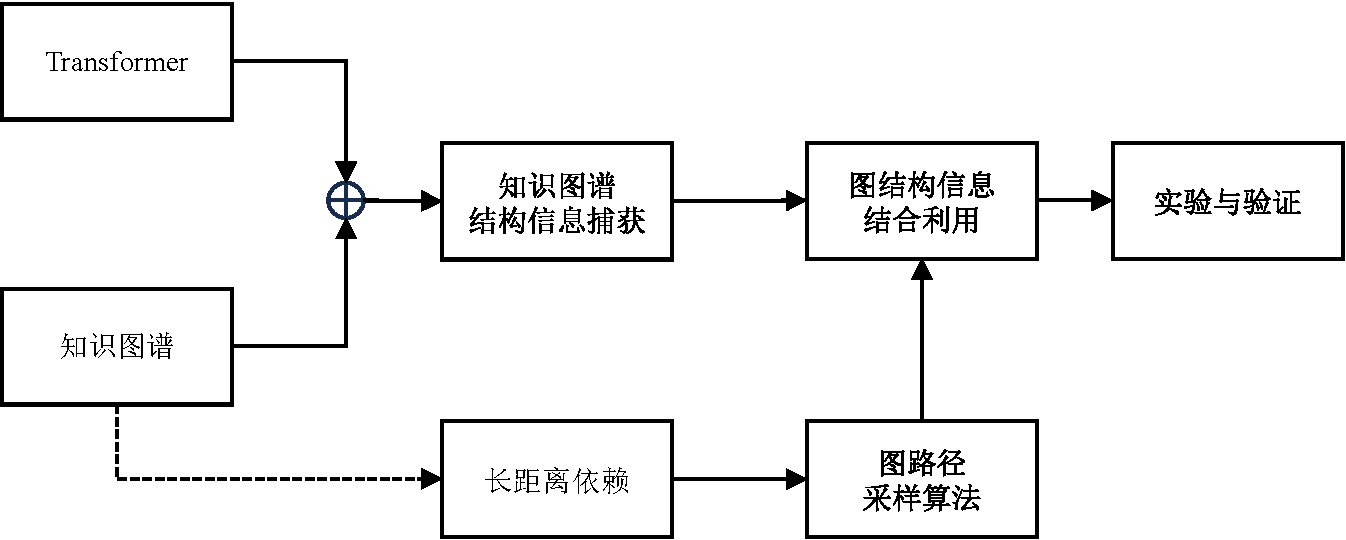
\includegraphics[width=0.9\textwidth]{pic/research_route_2.pdf}}
  \caption{研究路线示意图}
  \label{research_route}
\end{figure}

(1)基于Transformer的模型对于知识图谱结构的捕获研究

在Transformer中,任意一个位置都能直接感知到其他位置的输入信息,这导致模型无法直接捕捉到输入之间的相对位置关系,因此在处理序列数据时,采用的方式一般是为每个位置的输入添加对应的位置编码,标识输入与输入之间的前后位置关系。但在知识图谱中节点并不是顺序排列的,因此本文的主要研究内容之一就是设计一种合适方案让Transformer模型能够学习到知识图谱的拓扑结构,实现对知识图谱结构的感知。此外,在知识图谱中关系也是重要的结构信息,反映着实体和实体之间不同的交互方式,蕴含着丰富的语义信息,但标准的Transformer模型并没有直接的方式来编码和使用边的信息,因此Transformer如何对边信息进行表示也是重要的研究内容。

(2)图路径采样算法研究

针对基于图神经网络的方法对知识图谱中长距离信息学习不足的缺陷,本文计划通过对知识图谱中的图路径信息学习来挖掘实体与实体之间的长距离依赖,因此为了提升模型性能,对于当前的待遇测事实三元组,如何采样到高质量的图路径是首先需要解决的问题。因此本文计划研究设计合适的采样策略,实现高效的图路径采样,提高模型捕获长距离依赖的能力。

(3)不同图结构信息的结合方案研究

基于图神经网络的模型通过聚合消息的方式实现了对于中心实体局部邻域结构的感知,但无法捕捉实体之间长距离的依赖;基于图路径的方法能够挖掘到更远距离的依赖,但忽略了实体丰富的局部邻域。因此,本文的主要研究内容之一是设计合适的模型结构实现对于以上两类图结构信息的综合利用,实现对于图谱中长短距离信息的捕捉。

(4)实验与验证

在完成以上研究内容,实现完整的知识图谱补全模型之后,设计相应实验方案,通过平均排名、平均倒数排名等指标在主流公开数据集上与基线模型进行性能对比,验证本文提出的模型的有效性;并且通过设计合适的消融实验,验证模型关键设计的有效性。

\subsection{论文组织安排}
本文对基于Transformer的知识图谱补全方法进行研究,论文内容总共分为五个章节以及总结与展望部分,各个章节的内容安排组织如下:

第一章绪论首先介绍了论文的背景与意义,随后对知识图谱以及知识图谱算法的国内外研究进展进行了简单介绍,并进行了各类方法的对比与总结。随后明确了论文的研究目标与研究路线,概述了论文的主要研究内容。最后介绍了论文的组织安排。

第二章介绍了论文中方法所涉及到的相关理论基础。首先介绍了注意力机制与Transformer模型架构,其次对Transformer模型在图学习领域中的应用进行了概述,最后对不同类别的知识图谱嵌入方法进行了介绍,包括部分模型的核心思想以及数学公式。

第三章首先对Transformer模型在知识图谱嵌入领域的应用存在的困难进行了分析,随后介绍了提出的基于邻域感知Transformer的知识图谱补全模型,给出了符号定义以及模型的总体架构,并对其中的关键设计结构强化的自注意力机制进行了说明。

第四章首先指出了现有的基于图结构信息的方法的缺点,随后介绍了提出的结合图路径和局部邻域的Transformer知识图谱嵌入模型,说明了模型的总体架构以及各个模块的设计方案,包括基于有偏随机游走的图路径采样算法、图路径信息与局部邻域信息的结合方案以及掩蔽实体关系预测任务。

第五章为实验与验证部分,首先说明了实验采用的数据集、选取的进行对比的基线模型、实验环境以及采用的评估策略等基本情况,随后对实验结果进行了介绍和分析,包括本文提出的模型与基线模型的总体性能对比、关键模块消融实验的结果,超参数对于模型的性能影响等。

总结与展望部分对本文的研究内容进行了回顾与总结,并对未来可能的研究方向进行了展望。

\input{tex/chap_intro}

% 说明
\input{tex/chap_instruction}

% 示例
\input{tex/chap_sample}

% 总结
% !TeX root = ../Template.tex
% 总结
\summary
% 自从2017年被提出,Transformer已经在计算机视觉、自然语言处理等多个领域大放异彩,展现出了巨大的潜力,收到了许多的关注,因此也有不少工作尝试将Transformer网络引入到知识图谱补全领域中。
本课题针对传统知识图谱嵌入方法和基于图神经网络的方法的缺点,研究如何利用Transformer模型来学习知识图谱中的语义和结构信息,提升知识图谱补全任务的性能,提出了两种新型的基于Transformer的知识图谱补全方法:基于邻域感知的Transformer模型NATLP,并在NATLP模型的基础上进一步提出了结合图路径和局部邻域的Transformer模型TKGE-PN。

针对基于图神经网络的知识图谱嵌入方法表达能力不足的问题,NATLP研究利用Transformer网络来完成知识图谱补全。针对以往模型对关系和实体间的交互建模不足的问题,NATLP在模型输入信息构造阶段,基于关系生成特定的网络参数,实现关系特定的邻居信息构造,显示建模了不同关系对于实体传递消息的影响;针对Transformer无法直接感知图结构的问题,NALTP对Transformer的自注意力机制进行了改造,提出了一种融合图结构的自注意力机制,使得模型能够学习到输入消息之间的互相依赖;

NATLP模型解决了基于图神经网络的模型存在的部分问题,但依然无法有效学习图谱中的长距离依赖。针对基于图神经网络的方法和NATLP方法中的以上缺陷,本文在NATLP的基础上进一步提出了结合图路径和局部邻域的Transformer模型TKGE-PN。TKGE-PN通过对知识图谱中的局部邻域和图路径两种结构信息的融合,完成了在利用丰富的邻域信息的同时对于图谱中长距离信息的挖掘,提高了知识图谱补全任务的性能。TKGE-PN首先通过基于有偏随机游走的采样算法对图路径进行采样,随后通过基于Transformer的图路径编码模块学习其中的长距离依赖,并通过掩蔽实体关系任务实现长短距离信息的平衡;最后通过局部邻域编码模块实现了图路径和局部邻域结构信息的综合应用。

实验结果表明,在两个标准数据集WN18RR和FB15k-237上,NATLP和TKGE-PN的链路预测任务的性能表现超越绝大多数现有的嵌入模型,证明了本文提出的两个模型以及其中的关键设计的有效性。

% 未来,我们计划进一步探索对于知识图谱中结构信息的利用,包括更有效率的利用方式和更加丰富的结构信息种类,同时尝试将TKGE-PN应用到除链路预测之外的其他知识图谱表示学习任务中。

本文涉及的研究内容还有许多可以拓展的地方。首先,知识图谱的图结构除了图路径和局部邻域之外还有其他的表现形式,我们计划进一步探索对于知识图谱中结构信息的利用,例如在规模更大的子图范围上来应用Transformer网络,进一步挖掘模型的潜力。

其次,除了结构信息之外,知识图谱中也蕴含着丰富的文本信息,例如实体的文字描述。而Transformer网络被广泛应用于预训练语言模型中,在挖掘文本语义信息方面存在天然优势。未来我们计划研究将模型与预训练语言模型进行结合,同时利用文本信息和图结构信息来完成知识图谱补全任务。

最后,Transformer网络的复杂度较高,训练和预测时的开销较大,在处理大规模知识图谱时可能会遇到资源上的瓶颈。因此如何优化基于Transformer的结构带来的大量资源开销也是一个值得研究的方向。



% 参考文献
% 手册中参考文献标准似乎并没有严格按照国标GBT7714-2015执行
\Bib{bst/GBT7714-BUAA}{ref}

% 附录
\input{tex/chap_appendix}

% 攻读学位期间成果
% !TeX root = ../Template.tex
% [攻读学位期间取得的成果]
\achievement
\noindent
[1] Liu X, \textbf{Zhu T}, Tan H, et al. Heterogeneous graph neural network with hypernetworks
for knowledge graph embedding [C]//The Semantic Web–ISWC 2022: 21st International
Semantic Web Conference, Virtual Event, October 23–27, 2022, Proceedings. Berlin,
Heidelberg: Springer-Verlag, 2022: 284–302

\noindent
[2] 郭子溢,\textbf{朱桐},林广艳,等. 球面坐标下基于语义分层的知识图谱补全方法 [J]. 应用科学学报, 2024, 42 (01): 119-133.



% 致谢
% !TeX root = ../Template.tex
% [致谢]
\acknowledgments

研究生三年生涯转瞬即逝,我的学生生涯也马上要走到了尽头。回首过去的三年,我初次叩开了科研的大门,虽然未能深入探索,但也收获良多,受益匪浅。

在三年的研究生生活中,我首先要感谢的是谭火彬老师和林广艳老师对我的学术和生活上给予的指导和帮助。两位老师不仅会在学术上为我提供建议,指明方向,对我的论文提出了许多宝贵的修改意见,生活中,还时刻关心着我们的身体健康和心理状况,在我的职业规划上也提供了大力的支持。实验室的良好氛围也为我提供了非常好的学习和研究的环境。能够接受两位老师的指导是我的幸运。还要感谢我的父母,他们的默默付出是我最坚强的后盾,父母的理解和爱护是我低谷时最重要的慰藉和支持。

此外,我还要感谢实验室的各位同门。感谢刘希阳学长在我初入实验室时提供的指导,帮助我迈出了学术研究的第一步,在我论文工作遇到困难时也对我提出了非常宝贵的意见和建议。还要感谢柳啸峰、郭子溢、朱伯同三位学长在我的学术研究中为我答疑解惑,学长们丰富的经验帮助我少走了不少弯路。感谢任博林和蒋沛宇两位学弟,论文实验的顺利完成离不开他们对于实验室服务器的维护。

最后,我要感谢我的小伙伴们,三年的时间我们一起度过了一段难忘的时光。




% 作者简介
\input{tex/chap_biography}

\vspace{5cm}

This is \BUAAThesis{}, Happy TeXing! --- from WeiQM.

\end{document}
